
%En ella se deben exponer brevemente pero con absoluta claridad, 
% la novedad y actualidad del tema,
% el objeto de la investigaci�n,
% sus objetivos,
% la hip�tesis de trabajo,
% el fundamento metodol�gico y
% los m�todos utilizados para realizar el trabajo de investigaci�n.
%Es decir, que la introducci�n es la fundamentaci�n cient�fica de la tesis en forma resumida.

\section{Introduction}
\begin{frame}

  The aim of this thesis is to support decision making concerning to
  the location and redeployment of insurance agents to attend road accidents.

  The methods of solution that will be proposed to will be improve the service
  offered by insurance agents, helping them to reach in less time,
  or determine the number of adjusters required to perform the service within
  the desired standards.
\end{frame}

\subsection{Problem}
\begin{frame}

  \textit{Determine the optimal bases (locations)
  for adjusters available, 
  so that the average response time
  to claims incurred in a given region,
  whether in the shortest possible time}
\end{frame}

\subsection{Motivation}
\begin{frame}
  When a car accident occurs, 
  it begins to increase traffic congestion on surrounding roads.
  This because the presence of an adjuster (proficient)
  which record and determine the causes of the accident,
  in order to move the car from the accident area and restore the flow.
  \begin{center}
    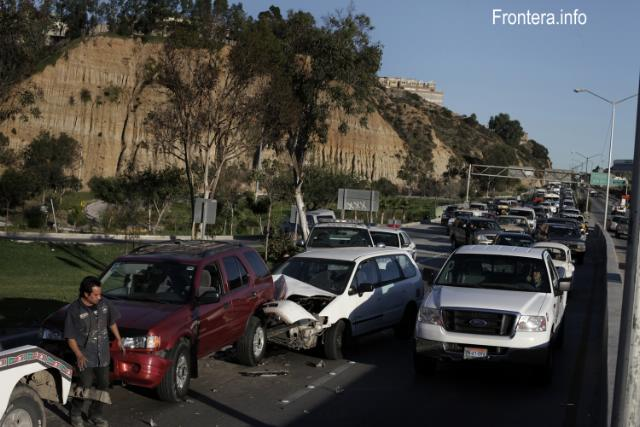
\includegraphics[scale=0.25]{389200-G}
  \end{center}
\end{frame}

\subsection{Background}
\begin{frame}[allowframebreaks]
  Richard C. Larson (1974) \cite{larson1974hypercube} 
  proposes the hyper-cube model.

  James P. Jarvis (1985) \cite{jarvis1985approximating} incorporates
  location dependent service times characteristics,
  developing an approximation model for a spatially distributed queuing system
  under general service time assumptions.

  Berman, Larson et. al (1987) \cite{berman1987stochastic}
  formulates the stochastic queue p-median problem,
  and propose a heuristic approach for locating cooperative service facilities
  on a network.

  Goldberg et. al (1990) \cite{goldberg1990validating}
  proposes a nonlinear integer programming
  model for finding optimal base locations for emergency medical vehicles.

\end{frame}
